\documentclass[aspectratio=169]{beamer}

\usepackage[utf8]{inputenc}
\usepackage[T1]{fontenc}
\usepackage[spanish]{babel}
\usepackage{lmodern}
\usepackage{amsmath,amssymb}
\usepackage{graphicx}
\usepackage{booktabs}
\usepackage{array}
\usepackage{tikz}
\usetikzlibrary{babel,arrows.meta,positioning}
\usepackage{listings}
\graphicspath{{figs/}}

\usetheme{Madrid}
\usecolortheme{seahorse}
\setbeamertemplate{navigation symbols}{}
\setbeamerfont{frametitle}{size=\large}

% Divisor de sección: una slide con el título de la sección que comienza
\setbeamertemplate{section page}{
  \centering
  {\usebeamercolor[fg]{structure}\large Sección \insertsectionnumber\par}
  \vspace{3mm}
  \begin{beamercolorbox}[sep=12pt,center,rounded=true,shadow=true]{title}
    \usebeamerfont{title}\insertsectionhead\par
  \end{beamercolorbox}
}
\AtBeginSection[]{
  \begin{frame}[plain,noframenumbering]
    \sectionpage
  \end{frame}
}

\title[Gas 3D con LGA híbrido]{Expansión de un gas 3D con autómata celular\\y paralelismo híbrido BSPlib + OpenMP}
\subtitle{Sistema, reglas del autómata y paralelización híbrida}
\author[Ahumada, Muñoz]{Gonzalo Ahumada \and Daniel Muñoz}
\institute[USACH]{Laboratorio 2 --- High Performance Computing\\[1mm]
           Universidad de Santiago de Chile}
\date{\today}

\begin{document}

\begin{frame}
  \titlepage
\end{frame}

% ---------------------------------------------------------------------------
\section{El sistema}
% ---------------------------------------------------------------------------

\begin{frame}{Problema}
  \begin{itemize}
    \item Simular la \alert{expansión de un gas en 3D} sobre una malla cúbica.
    \item Usar un \alert{autómata celular} con reglas locales y estado finito.
    \item Mostrar \alert{paralelismo híbrido}: procesos (BSPlib) + hilos
          (OpenMP).
    \item Requisitos del curso:
      \begin{itemize}
        \item C++, BSPlib para procesos y OpenMP para hilos,
        \item ejecución exigente pero posible en un PC,
        \item objetivo de referencia $4$ procesos $\times$ $8$ hilos,
        \item entregables: código, informe y presentación.
      \end{itemize}
    \item Desafío: comunicación regular, conservación exacta y \emph{scaling}
          en una carga \emph{memory-bound}.
  \end{itemize}
\end{frame}

\begin{frame}{Gas ideal: neón a 1 atm y 300 K}
  \begin{columns}[T]
    \begin{column}{0.53\textwidth}
      \begin{itemize}
        \item Partículas puntuales, sin fuerzas de largo alcance.
        \item Colisiones binarias elásticas.
        \item Gas noble monoatómico: $\gamma=5/3$, sin modos internos.
        \item A 1 atm y 300 K la corrección del virial es
              \alert{0.05\%}: el gas ideal basta.
      \end{itemize}
    \end{column}
    \begin{column}{0.45\textwidth}
      \begin{block}{Decisión}
        \footnotesize
        \alert{Neón} como gas ideal. La presión sale de la densidad del
        autómata: $p=\tfrac{\rho}{3}\,p_0$, con $p_0=1$ atm.
      \end{block}
      \begin{alertblock}{Limitación declarada}
        \footnotesize
        El autómata es \alert{isotérmico}: no captura el enfriamiento
        adiabático. El foco es HPC y la forma de la expansión.
      \end{alertblock}
    \end{column}
  \end{columns}
\end{frame}

\begin{frame}{Condición inicial: cámara de dos presiones}
  \begin{columns}[T]
    \begin{column}{0.50\textwidth}
      \centering
      \begin{tikzpicture}[font=\scriptsize,scale=0.95]
        \draw[->] (0,0) -- (6.4,0) node[right] {$x$};
        \draw[->] (0,0) -- (0,2.5) node[above] {$\rho$};
        \draw[thick] (0,2) -- (1.9,2) -- (2.8,0.4) -- (6.2,0.4);
        \draw[dashed] (1.9,0) -- (1.9,2);
        \draw[dashed] (2.8,0) -- (2.8,0.4);
        \node at (0.8,2.2) {$\rho_H$};
        \node at (5.5,0.65) {$\rho_L$};
        \node at (2.35,1.2) {rampa};
        \node at (1.9,-0.25) {$x_i$};
      \end{tikzpicture}
    \end{column}
    \begin{column}{0.48\textwidth}
      \begin{block}{Valores}
        \footnotesize
        \begin{itemize}
          \item $p_H=1$ atm ($\rho_H=3$) para $x<0.25N$.
          \item $p_L=0.1$ atm ($\rho_L=0.3$) en el resto.
          \item Razón $10{:}1$, rampa de $w=8$ celdas.
        \end{itemize}
      \end{block}
      \begin{block}{Por qué}
        \footnotesize
        Gradiente de presión explícito y una onda de expansión medible.
        Una \alert{esfera densa} en vacío queda como caso base.
      \end{block}
    \end{column}
  \end{columns}
\end{frame}

% ---------------------------------------------------------------------------
\section{Reglas del autómata celular}
% ---------------------------------------------------------------------------

\begin{frame}{Estado del autómata}
  \begin{columns}[T]
    \begin{column}{0.52\textwidth}
      \begin{itemize}
        \item Malla $N\times N\times N$.
        \item 6 bits por celda: $\pm x,\pm y,\pm z$.
        \item Exclusión: máximo una partícula por dirección.
        \item 64 estados posibles (\texttt{uint8\_t}).
        \item Estado entero $\Rightarrow$ conservación exacta.
      \end{itemize}
      \begin{block}{Decisión}
        \footnotesize
        6 direcciones, \alert{sin partícula en reposo}: modelo 3D mínimo,
        1 byte por celda y suficiente para una expansión cualitativa.
      \end{block}
    \end{column}
    \begin{column}{0.44\textwidth}
      \centering
      \begin{tikzpicture}[>=Stealth,font=\small,scale=0.9]
        \node[draw,circle,fill=blue!10,minimum size=8mm] (c) at (0,0) {celda};
        \draw[->,thick] (c) -- (1.1,0)  node[right] {$+x$};
        \draw[->,thick] (c) -- (-1.1,0) node[left]  {$-x$};
        \draw[->,thick] (c) -- (0,1.1)  node[above] {$+y$};
        \draw[->,thick] (c) -- (0,-1.1) node[below] {$-y$};
      \end{tikzpicture}
      \vspace{2mm}
      {\scriptsize $\pm z$: fuera del plano}
    \end{column}
  \end{columns}
\end{frame}

\begin{frame}{Reglas: colisión y streaming}
  \begin{block}{Colisión}
    \footnotesize
    Agrupar estados por $(M,P_x,P_y,P_z)$ y mapear cada uno a otro del mismo
    grupo:
    \[
      M(s')=M(s),\qquad \vec{P}(s')=\vec{P}(s).
    \]
    8 tablas elegidas por celda con un hash global.
  \end{block}
  \begin{block}{Streaming}
    \footnotesize
    Cada bit se mueve a la celda vecina. Formulación \emph{gather}:
    \[
      s^{t+1}_{x,y,z}=(s^t_{x-1,y,z}\wedge B_{+x})
      \vee(s^t_{x+1,y,z}\wedge B_{-x})\vee\cdots
    \]
  \end{block}
  \begin{alertblock}{Invariantes}
    \footnotesize
    Masa y momento total se conservan \alert{exactamente}: estado entero y
    reglas locales, un autómata celular estricto y sin errores de redondeo.
  \end{alertblock}
\end{frame}

\begin{frame}{Ejemplo: un paso del autómata}
  \centering
  \begin{tikzpicture}[>=Stealth,font=\scriptsize]
    \foreach \ox/\lab in {0/Antes, 4.0/Tras la colisión, 8.0/Tras el streaming} {
      \begin{scope}[shift={(\ox,0)}]
        \node at (1.2,2.75) {\small\textbf{\lab}};
      \end{scope}
    }
    % panel 1: choque frontal en x
    \fill[blue!10] (0.8,0.8) rectangle (1.6,1.6);
    \draw[gray!60] (0,0) grid[step=0.8] (2.4,2.4);
    \draw[->,very thick,red] (1.2,1.2) -- ++(0.36,0);
    \draw[->,very thick,red] (1.2,1.2) -- ++(-0.36,0);
    \node[align=center] at (1.2,-0.45) {$+x$ y $-x$\\masa 2, momento 0};
    % flecha colisión
    \draw[->,thick] (2.7,1.2) -- node[above] {colisión} (3.7,1.2);
    % panel 2: salen en y
    \begin{scope}[shift={(4.0,0)}]
      \fill[blue!10] (0.8,0.8) rectangle (1.6,1.6);
      \draw[gray!60] (0,0) grid[step=0.8] (2.4,2.4);
      \draw[->,very thick,blue] (1.2,1.2) -- ++(0,0.36);
      \draw[->,very thick,blue] (1.2,1.2) -- ++(0,-0.36);
      \node[align=center] at (1.2,-0.45) {$+y$ y $-y$\\masa 2, momento 0};
    \end{scope}
    % flecha streaming
    \draw[->,thick] (6.7,1.2) -- node[above] {streaming} (7.7,1.2);
    % panel 3: cada partícula avanza a la vecina
    \begin{scope}[shift={(8.0,0)}]
      \fill[blue!10] (0.8,1.6) rectangle (1.6,2.4);
      \fill[blue!10] (0.8,0.0) rectangle (1.6,0.8);
      \draw[gray!60] (0,0) grid[step=0.8] (2.4,2.4);
      \draw[->,very thick,blue] (1.2,2.0) -- ++(0,0.36);
      \draw[->,very thick,blue] (1.2,0.4) -- ++(0,-0.36);
      \node[align=center] at (1.2,-0.45) {cada partícula pasa\\a la celda vecina};
    \end{scope}
  \end{tikzpicture}
  \vspace{4mm}
  \begin{block}{Cómo se lee}
    \footnotesize
    Dos partículas chocan de frente. La tabla de la celda elige la salida
    entre $\pm x$, $\pm y$ y $\pm z$: todas tienen \alert{la misma masa y el
    mismo momento}. Luego cada partícula avanza una celda en su dirección.
    {\scriptsize (Vista en el plano $x$--$y$; en 3D se suma $\pm z$.)}
  \end{block}
\end{frame}

% ---------------------------------------------------------------------------
\section{Paralelización híbrida}
% ---------------------------------------------------------------------------

\begin{frame}{La idea: dividir el cubo en dos niveles}
  \begin{columns}[T]
    \begin{column}{0.56\textwidth}
      \centering
      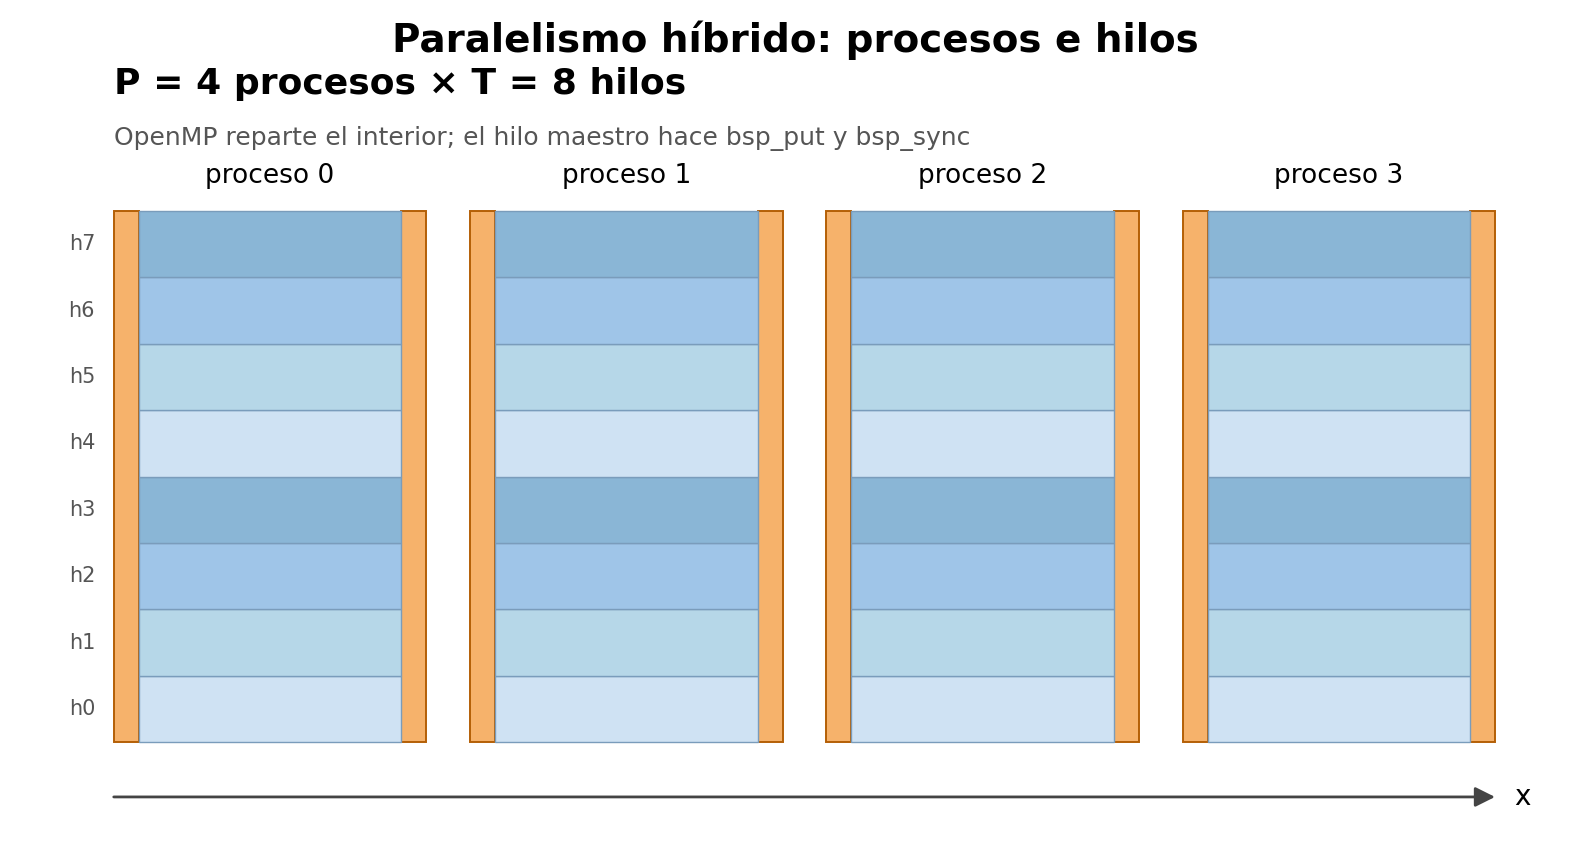
\includegraphics[width=\textwidth]{hybrid_4x8.png}
    \end{column}
    \begin{column}{0.42\textwidth}
      \begin{block}{Procesos (BSPlib)}
        \footnotesize
        El cubo se corta en $P=4$ bloques de capas en $x$. Cada proceso tiene
        \alert{su propia memoria}: no ve los datos de los otros.
      \end{block}
      \begin{block}{Hilos (OpenMP)}
        \footnotesize
        Dentro de cada bloque, $T=8$ hilos se reparten las celdas.
        \alert{Comparten memoria}: no necesitan mensajes.
      \end{block}
      \begin{block}{Resultado}
        \footnotesize
        $4\times8=32$ hilos trabajando a la vez.
      \end{block}
    \end{column}
  \end{columns}
\end{frame}

\begin{frame}{Un paso de simulación = un superpaso BSP}
  \begin{columns}[T]
    \begin{column}{0.44\textwidth}
      \begin{enumerate}
        \footnotesize
        \item \alert{Calcular} colisiones \hfill {\scriptsize (OpenMP)}
        \item \alert{Enviar bordes}: la capa del borde va al ghost del vecino
              \hfill {\scriptsize (\texttt{bsp\_put})}
        \item \alert{Esperar a todos} \hfill {\scriptsize (\texttt{bsp\_sync})}
        \item \alert{Mover} partículas \hfill {\scriptsize (OpenMP)}
      \end{enumerate}
      \vspace{2mm}
      \begin{alertblock}{Regla de seguridad}
        \footnotesize
        BSPlib no es thread-safe: solo el \alert{hilo maestro} envía y
        sincroniza, fuera de las regiones OpenMP.
      \end{alertblock}
    \end{column}
    \begin{column}{0.54\textwidth}
      \centering
      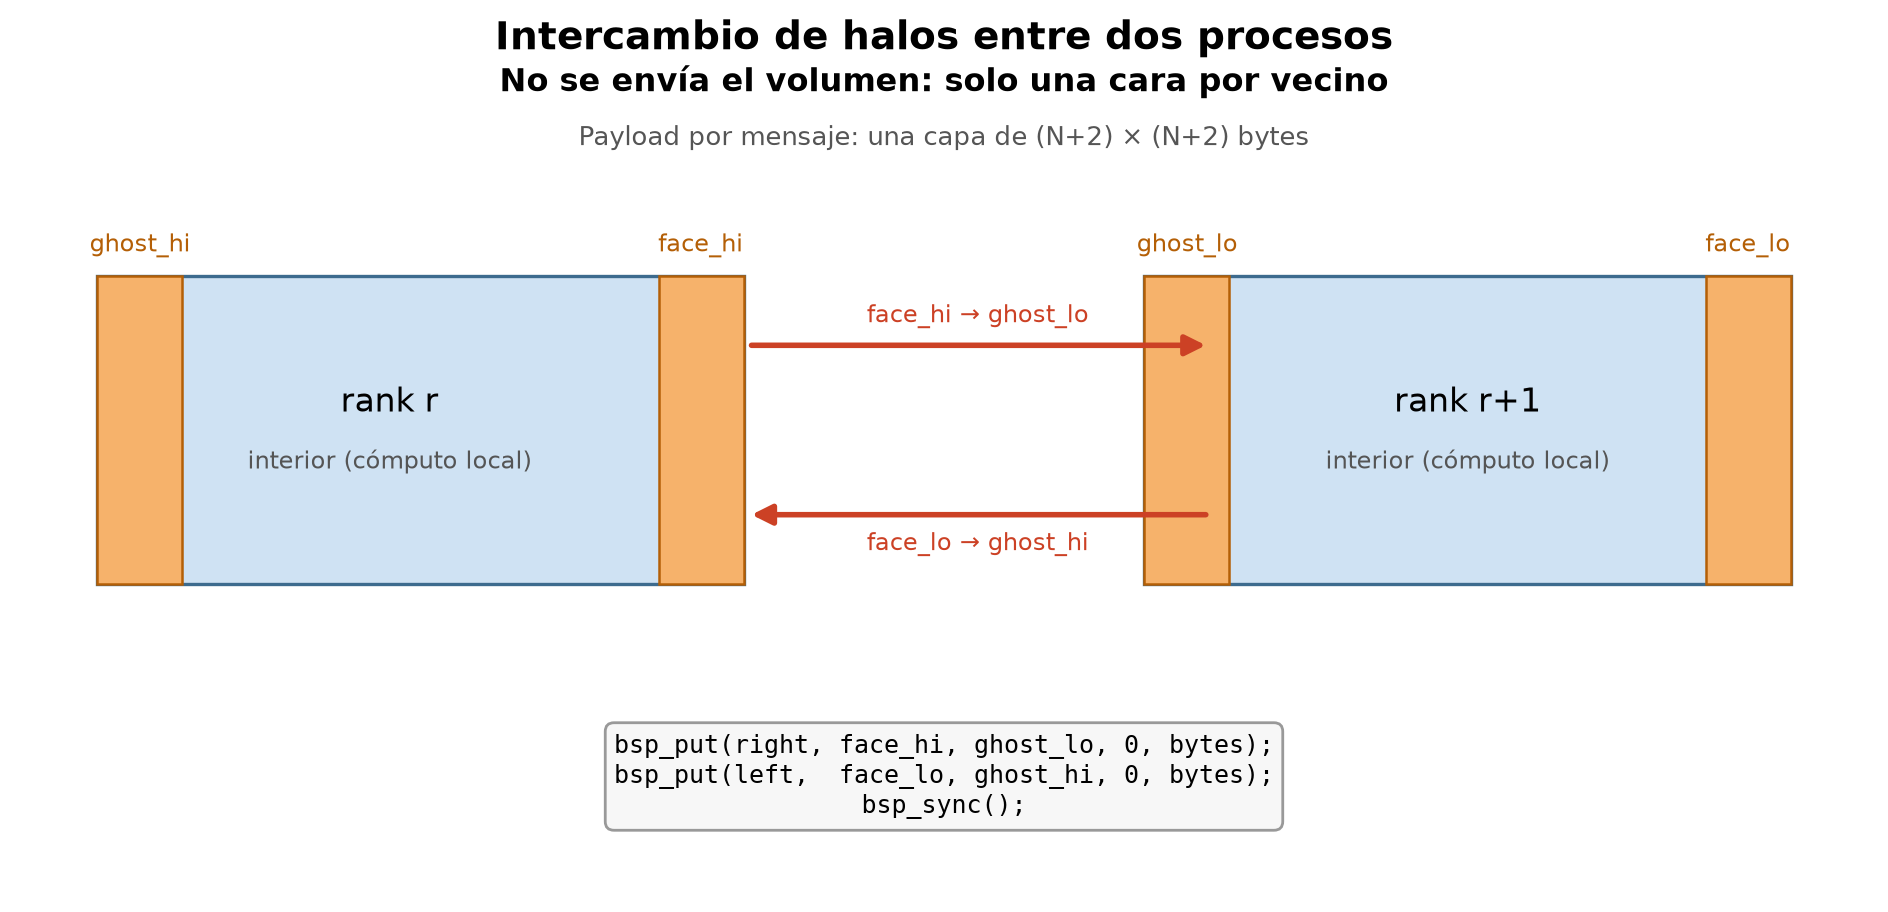
\includegraphics[width=\textwidth]{halo_exchange.png}\par
      {\scriptsize Solo se envía una cara por vecino, no el volumen.}
    \end{column}
  \end{columns}
\end{frame}

\begin{frame}{Cuánto cuesta un superpaso}
  \begin{block}{Modelo de costo BSP aplicado a nuestro paso}
    \[
      T_{\text{paso}} \;=\;
      \underbrace{\tfrac{N}{P}\,N^2\, t_c}_{w:\ \text{calcular (volumen)}}
      \;+\;
      \underbrace{2\,(N+2)^2\, g}_{h\cdot g:\ \text{bordes (superficie)}}
      \;+\;
      \underbrace{L}_{\text{barrera}}
    \]
  \end{block}
  \begin{itemize}
    \footnotesize
    \item $t_c$: costo de actualizar una celda; $g$: costo por byte enviado;
          $L$: costo de sincronizar.
    \item El cálculo crece con el \alert{volumen} ($N^3$); la comunicación con
          la \alert{superficie} ($N^2$).
    \item Razón comunicación / cálculo $\;\approx\; \dfrac{2P}{N}$.
  \end{itemize}
  \begin{alertblock}{Idea clave}
    \footnotesize
    Mientras más grande el cubo, menos pesa la comunicación: el problema debe
    ser grande para que $4\times8$ valga la pena.
  \end{alertblock}
\end{frame}

\begin{frame}{Por qué un problema grande: $N=1024$}
  \centering
  \footnotesize
  \begin{tabular}{lrr}
    \toprule
    $P=4$, $T=8$ & $N=256$ & $N=1024$ \\
    \midrule
    Comunicación / cálculo ($2P/N$) & 3.1\,\% & 0.8\,\% \\
    Celdas por hilo & 0.5 M & 33.5 M \\
    Halo enviado por proceso y paso & 133 KB & 2.1 MB \\
    Memoria total (2 buffers) & 33 MB & 2.1 GB \\
    \bottomrule
  \end{tabular}
  \vspace{4mm}
  \begin{columns}[T]
    \begin{column}{0.48\textwidth}
      \begin{block}{$N=256$}
        \footnotesize
        Cada hilo tiene poco trabajo: la espera en la barrera pesa cada vez
        más frente al cálculo.
      \end{block}
    \end{column}
    \begin{column}{0.48\textwidth}
      \begin{block}{$N=1024$}
        \footnotesize
        Trabajo de sobra por hilo y comunicación despreciable:
        \alert{exigente pero posible en un PC}.
      \end{block}
    \end{column}
  \end{columns}
\end{frame}

\begin{frame}
  \centering
  \Huge Gracias\\[4mm]
  \normalsize ¿Preguntas?
\end{frame}

\end{document}
